\documentclass{article}
\usepackage{multicol}
\usepackage{graphicx} % Required for inserting images
\usepackage{amssymb}
\usepackage[margin=1in]{geometry}
\usepackage[T1]{fontenc}
\usepackage{hyperref}
\title{Not1MM User Manual}
\author{Mike Bridak K6GTE}
\date{October 2025}
\begin{document}
\maketitle
\thispagestyle{empty}
\pagestyle{empty}
\newpage
\tableofcontents
\newpage
\pagestyle{plain}
\setcounter{page}{1}
\section{Not1MM}
The worlds number 1 unfinished contest logger. \textsuperscript{*According to my daughter Corinna.}

\vspace{0.5cm}
Not1MM's interface is a blatant rip-off of N1MM. It is NOT N1MM and any problem you have with this software should in no way reflect on their software.
\subsection{Not1MM. What is it}
Not1MM attempts to be a usable amateur radio, or HAM, contest logger. It's written in Python 3.10+, and uses Qt6 framework for the graphical interface and SQLite for the database.
\subsection{The Why}
\textbf{Currently, this exists for my own personal enjoyment}. I recently retired after 35+ years working for 'The Phone Company', GTE → Verizon → Frontier. And being a Gentleman of Leisure, I needed something to do in my free time. I am a casual contester and could not find any contesting software for Linux that I wanted to use. There is \textbf{Tucnak}, available at \emph{HTTP://tucnak.nagano.cz/} which is very robust and mature. It just wasn't for me.
\subsection{Target Environment}
The primary target for this application is Linux. It may be able to run on other platforms, BSD and Windows. But I don't have a way, or desire, to directly support them. I've recently purchased an M4 Mac Mini, So I'll probably put more effort into that platform as well.
\subsection{Current State, or Code Maturity}
Not1MM is, at times, fairly stable. Recently, it would seem that I'm desperately trying to change that. The current focus of development is adding support for Multi Multi contest operations. It is something that I have no practical experience in. So you can expect the same quality of code fit and finish.
\newpage
\section{List of Should be Working Contests}
\begin{multicols}{3}
\begin{itemize}
    \item General Logging
    \item 10 10 Fall CW
    \item 10 10 Spring CW
    \item 10 10 Summer Phone
    \item 10 10 Winter Phone
    \item ARI 40 80
    \item ARI DX
    \item ARRL 10M
    \item ARRL 160M
    \item ARRL DX CW, SSB
    \item ARRL Field Day
    \item ARRL RTTY Roundup
    \item ARRL Sweepstakes
    \item ARRL VHF
    \item CQ 160
    \item CQ WPX
    \item CQ World Wide
    \item CWOps CWT, CWO
    \item DARC Xmas
    \item DARC VHF
    \item EA Majistad CW
    \item EA Majistad SSB
    \item EA RTTY
    \item ES FIELD DAY HF
    \item ES OPEN HF
    \item Helvetia
    \item IARU Field day
    \item IARU HF
    \item ICWC MST
    \item Japan International DX
    \item K1USN Slow Speed Test
    \item Labre RS Digi
    \item LZ DX
    \item NAQP
    \item Phone Weekly Test
    \item RAEM
    \item RAC Canada Day
    \item RandomGram
    \item REF CW, SSB
    \item SAC CW, SSB
    \item SPDX
    \item Stew Perry Top band
    \item UK/EI DX
    \item Weekly RTTY
    \item Work All Germany
    \item Winter Field Day
\end{itemize}
\end{multicols}
\subsection{Other not so Supported Contests}
Of note, state QSO parties. I haven't worked any yet. And no one has submitted a PR adding one... So there you go. In the near future I'll probably add California, guess where I live, and the 4 states QSO party.
\newpage
\section{Installation}
This section will hopefully get you started with installing Not1MM.
\subsection{Prerequisites}
Not1MM requires:
\begin{itemize}
    \item Python 3.10+
    \item PyQt6
    \item libportaudio2
    \item libxcb-cursor0 (maybe... Depends on the distro)
    \item libxslt-devel  (maybe... Depends on the distro)
    \item libxml2-devel  (maybe... Depends on the distro)
\end{itemize}
You should install these through your distribution's package manager before continuing.
\subsection{The Easy and Fast way to install or run the latest version}

Step 1. Visit https://docs.astral.sh/uv/ and install uv.

In short you run this in your terminal:
\begin{verbatim}
    •curl -LsSf https://astral.sh/uv/install.sh | sh
\end{verbatim}
Step 2. Tell it to run not1mm:
\begin{verbatim}
    •uvx not1mm@latest
\end{verbatim}
or install it:
\begin{verbatim}
    •uv tool install not1mm@latest
\end{verbatim}

That's it... It will go out, fetch the latest version of not1mm, setup a python virtual environment, get all the needed python libraries, cache everything and run not1mm. The first time takes a minute, but each time after, it's lightning quick and it will automatically check for updates and run the latest version.

But wait... There's more. If your distro is old and you're stuck with an older version of python... Say 3.10. And you want to see what all the cool kids are using. But you don't want to corrupt your broke ol' system by downloading the newest Python version. No problem. You can tell uv to run not1mm with any version of Python you'd like. Let's say 3.14.

\begin{verbatim}
    •uvx --python 3.14 not1mm@latest
\end{verbatim}

It'll download Python 3.14 into you virtual environment and run not1mm. Let's say I was an idiot and pushed a new version and did't fully test it. This happens a-lot... We test in production. Or lets say you just want to see the pain that was back in 2023. No problem. Just tell it which version of not1mm you'd like to run.

\begin{verbatim}
    •uvx --python 3.10 not1mm==23.5.19
\end{verbatim}

Pow! Enjoy the pain... 
\newpage
\section{After the Install}
You can now open a new terminal and type `not1mm`. On it's first run, it may or may not install a lovely non AI generated icon, which you can later click on to launch the application.

\subsection{You May or May Not Get a Warning Message Like}

\begin{verbatim}
WARNING: The script not1mm is installed in '/home/mbridak/.local/bin',
which is not on PATH. Consider adding this directory to PATH or,
if you prefer to suppress this warning, use --no-warn-script-location.
\end{verbatim}

If you do, log out and back in or reboot.

\subsection{Or this Fan Favorite}

\begin{verbatim}
Warning: Ignoring XDG\_SESSION\_TYPE=wayland on Gnome.
Use QT\_QPA\_PLATFORM=wayland to run on Wayland anyway.
qt.qpa.plugin: Could not load the Qt platform plugin "xcb"
even though it was found. This application failed to start
because no Qt platform plugin could be initialized.
Reinstalling the application may fix this problem.
\end{verbatim}

You can use your package manager to load \textbf{libxcb-cursor0}.\\
If that is not an option, you can export an environment variable and launch the app like this:

\begin{verbatim}
mbridak@vm:~$ export QT_QPA_PLATFORM=wayland; not1mm
\end{verbatim}

For a more permanent solution, you can place the line:

\begin{verbatim}
export QT_QPA_PLATFORM=wayland
\end{verbatim}

in your home directories .bashrc file. Then after logging out and back in you should be able to launch it normally.

\subsection{Update Your CTY and SCP Files}

Before operating in a contest, you might want to update the CTY and SCP files. You can do this by choosing \textbf{FILE >> Update CTY} and \textbf{FILE >> Update MASTER.SCP}
\newpage
\section{Various Data File Locations}

\subsection{Data}

If your system has an `XDG\_DATA\_HOME` environment variable set, the database and CW macro files can be found there. Otherwise they will be found at `yourhome/.local/share/not1mm`

\subsection{Config}

Configuration file(s) can be found at the location defined by
\begin{verbatim}XDG_CONFIG_HOME\end{verbatim}
Otherwise they will be found at \begin{verbatim}yourhome/.config/not1mm\end{verbatim}
\section{The Database}

\subsection{Why}

The database holds... wait for it... data... I know shocker right. A database can hold one or many contest logs. It also holds the station information, everything shown in the Station Settings dialog. You can have one database for the rest of your life. Filled with hundreds of contests you've logged. Or, you can create a new database to hold just one contest. You do You Boo.

\subsection{The First One is Free}

On the initial running, a database is created for you called `ham.db`. This, and all future databases, are located in the data directory mentioned above.

\subsection{Why Limit Yourself}

You can create a new database by selecting \textbf{File >> New Database} from the main window, and give it a snazzy name. Why limit yourself. Hell, create one every day for all I care. You can manage your own digital disaster.

\subsection{Revisiting an Old Friend}

You can select a previously created databases for use by selecting
\textbf{File >> Open Database}.
\newpage
\section{Station Settings Dialog}

After initial run of the program or creating a new database you will need to fill out the Station Settings dialog that will pop up.

\vspace{0.5cm}
\includegraphics[width=0.9\linewidth]{pic/settings.png}
\vspace{0.5cm}

You can fill it out if you want to. You can leave our friends behind 'Cause your friends don't fill, and if they don't fill. Well, they're no friends of mine.

You can fill. You can fill. Everyone look at your keys. \emph{You had to be around in the 80's}

\subsection{Changing Station Information}

Station information can be changed any time by going to\\
\textbf{File >> Station Settings} and editing the information.

\section{Selecting a Contest}

\subsection{Selecting a New Contest}

Select \textbf{File >> New Contest}

\vspace{0.5cm}
\includegraphics[width=0.5\linewidth]{pic/new_contest.png}
\vspace{0.5cm}

\subsection{Selecting an Existing Contest as the Current Contest}

Select \textbf{File >> Open Contest}

\vspace{0.5cm}
\includegraphics[width=0.5\linewidth]{pic/select_contest.png}
\vspace{0.5cm}

\subsection{Editing Existing Contest Parameters}

You can edit the parameters of a previously defined contest by selecting it as the current contest. Then select \textbf{File >> Edit Current Contest}. Click `OK` to save the new values and reload the contest. `Cancel` to keep the existing parameters.

\section{Configuration Settings}

To setup your CAT control, CW keyer, Callsign lookups,
select \textbf{File >> Configuration Settings}

The tabs for groups and N1MM are disabled and are for future expansion.

\vspace{0.5cm}
\includegraphics[width=0.5\linewidth]{pic/configuration_settings.png}
\vspace{0.5cm}

\subsection{Lookup}

For callsign lookup, Two services are supported. QRZ and HamQTH. They require a username and password, Enter it here.

\subsection{Soundcard}

Choose the sound output device for the voice keyer.

\subsection{CAT Control}

Under the `CAT` TAB, you can choose either `rigctld` normally with an IP of `127.0.0.1` and a port of `4532`. Or `flrig`, IP normally of `127.0.0.1` and a port of `12345`. `None` is always an option, but is it really? There's an onscreen icon for CAT status. Green good, Red bad, Grey neither.

\subsection{CW Keyer Interface}

Under the `CW` TAB, There are three options. `cwdaemon`, which normally uses IP `127.0.0.1`port `6789`. `pywinkeyer` which normally uses IP `127.0.0.1` port `8000` and `CAT` which if your radio supports it, sends Morse characters via rigctld.

\subsection{Cluster}

\vspace{0.5cm}
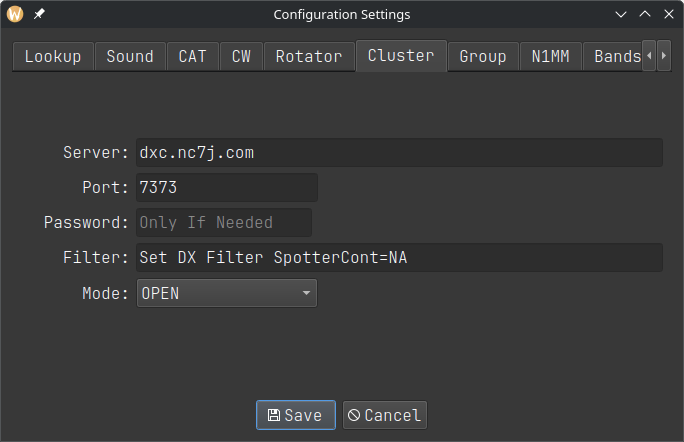
\includegraphics[width=0.9\linewidth]{pic/configuration_cluster.png}
\vspace{0.5cm}

Under the `Cluster` TAB you can change the default AR Cluster server, port and filter settings used for the bandmap window.

\subsection{N1MM Packets}

Work has started on N1MM UDP packets. So far just RadioInfo, contactinfo, contactreplace and contactdelete.

\vspace{0.5cm}
\includegraphics[width=0.9\linewidth]{pic/n1mm_packet_config.png}
\vspace{0.5cm}

When entering IP and Ports, enter them with a colon ':' between them. You can enter multiple pairs on the same line if separated by a space ' '.

\subsection{Bands}
You can define which bands appear in the main window. Those with checkmarks will appear. Those without will not.

\vspace{0.5cm}
\includegraphics[width=0.9\linewidth]{pic/configure_bands.png}
\vspace{0.5cm}

\subsection{Options}
On the Options TAB you can:
\begin{itemize}
\item Select to use Enter Sends Message (ESM), and configure it's function keys.
\item Select whether or not to use Call History info.
\item Select whether or not to send XML score info to online scoreboards.
\item Select whether or not to clear input fields when you QSY while in S\&P mode.
\end{itemize}

\vspace{0.5cm}
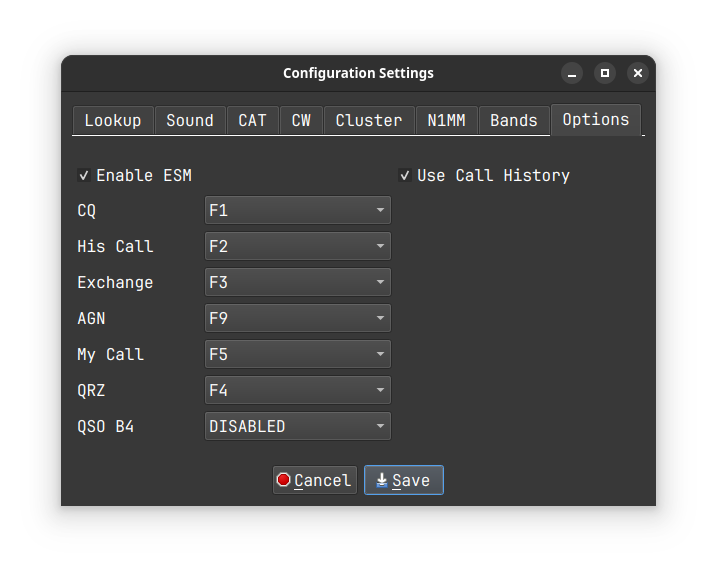
\includegraphics[width=0.9\linewidth]{pic/configuration_options.png}
\vspace{0.5cm}

Three realtime score boards are supported:
\begin{itemize}
\item Real Time Contest Server at hamscore.com
\item Contest Online ScoreBoard at contestonlinescore.com
\item iveScore at contest.run
\end{itemize}

\newpage
\section{Logging Digital Contacts}
Not1MM listens for WSJT-X UDP traffic on the Multicast address 224.0.0.1:2237. No setup is needed to be done on Not1MM's side. That's good because I'm lazy.\\Not1MM watches for fldigi qso's by watching for UDP traffic from fldigi on 127.0.0.1:9876.

\vspace{0.5cm}
\includegraphics[width=0.9\linewidth]{pic/fldigi_adif_udp.png}
\vspace{0.5cm}

The F1-F12 function keys are sent to fldigi via XMLRPC. Fldigi will be placed into TX mode, the message will be sent and a $\wedge$r will be tacked onto the end to place it back into RX mode.

Unlike WSJT, fldigi needs to be setup for this to work. The XMLRPC interface needs to be active. And in fldigi's config dialog, go to \textbf{CONTESTS >> General >> CONTEST} and select Generic Contest. Make sure the Text Capture Order field says CALL EXCHANGE.
\newpage
\section{Operating Multi Multi}

Work is underway on Multi Multi contest operations. There is a companion project \textbf{renfield}\\
\emph{https://github.com/mbridak/renfield} that will be needed for this. The idea is to have a separate slave server running, preferably, on another computer that's on the same network as the contesting PC's. This server will handle all the database CRUD operations. It will also handle the functions of handing out serial numbers and checking of a contact is a dupe. In the end, generating a Cabrillo file.

\vspace{0.5cm}
\begin{center}
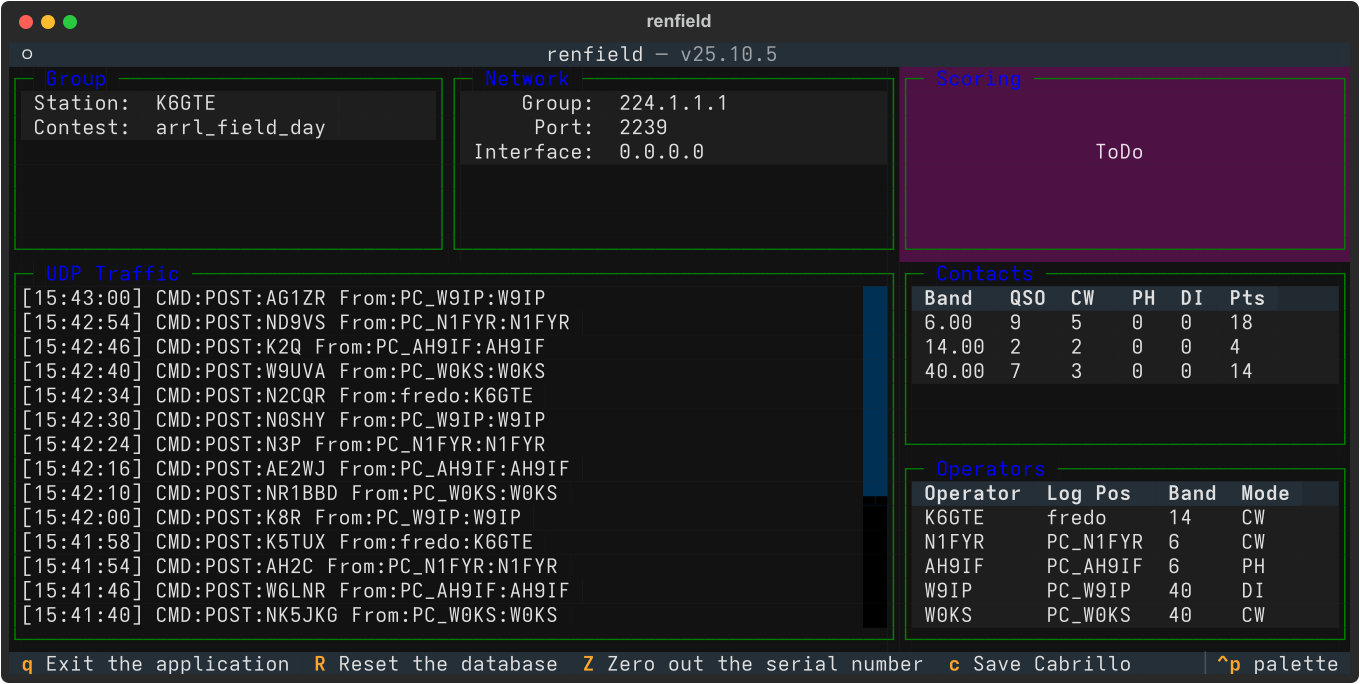
\includegraphics[width=0.75\linewidth]{pic/renfield_cli.png}
\end{center}
\vspace{0.5cm}

This is a very lightweight terminal application and can be easily hosted on a Raspberry Pi or similar device. In a pinch it can be run along side Not1MM on one of the contesting machines. Tho I'd think twice about that.

You could even use this while operating alone as an automated backup. So in case your logging computer should fail, you'd have a copy of the contest log.
\subsection{Network Settings for Multi Multi}
In the configuration dialog under the group tab, select Connect to server.

\vspace{0.5cm}
\begin{center}
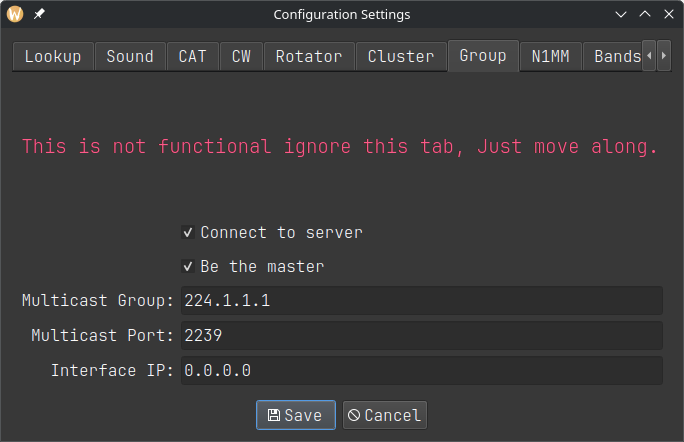
\includegraphics[width=0.5\linewidth]{pic/configuration_group.png}
\end{center}
\vspace{0.5cm}

One computer needs to be the master station. The master station will tell the renfield server what contest is being run.

\subsection{Contest Settings for Multi Multi}
For the settings of the contest, if the Operator is set to "MULTI-OP" and the Transmitter category is not "ONE" or "SWL" Not1MM will ask the renfield server for serial numbers and dupe checks.

\vspace{0.5cm}
\begin{center}
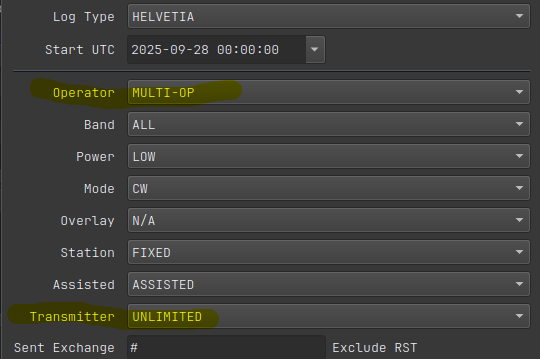
\includegraphics[width=0.5\linewidth]{pic/multi_multi.png}
\end{center}
\vspace{0.5cm}

\newpage
\section{Sending CW}
\subsection{Sending CW Macros}
Other than sending CW by hand, you can also send predefined CW text messages by pressing F1 - F12. See next section on Editing macro keys.
\subsection{Auto CQ}
If you press `SHIFT-F1` The Auto CQ mode will be activated, you will be placed in a Run state and the F1 macro will be resent after each Auto CQ Delay interval has passed. An indicator will appear to the upper left of the F1 macro key as a visual reminder that your Auto CQ is active. With it to the right, you will see a small progress bar giving you a visual indication as to when F1 will fire next.

\vspace{0.5cm}
\begin{center}
\includegraphics[width=0.25\linewidth]{pic/auto_cq_indicator.png}
\end{center}
\vspace{0.5cm}

\subsubsection{Setting the delay}
The delay can be changed by going to the `Options` TAB in the Configuration dialog. If you are in S\&P mode when you enable Auto CQ, you will be automatically switched into RUN mode. To properly set the delay you should time how long your F1 macro takes to key, then add how many seconds of pause you would like. This is your delay value.
\subsection{Sending CW Free Form}
If you need to send something freeform, you can press \textbf{CTRL-SHIFT-K}, this will expose an entry field at the bottom of the window which you can type directly into. When you're done you can either press \textbf{CTRL-SHIFT-K} again, or press the Enter Key to close the field.
\newpage
\section{Editing Macro Keys}
To edit the macros, choose \textbf{File >> Edit Macros}. This will open your systems registered text editor with current macros loaded. When your done just save the file and close the editor. The file loaded to edit, CW, SSB or RTTY, will be determined by your current operating mode and contest. Each contest gets it's own copy of the macros.

After editing and saving the macro file. You can force the logger to reload the macro file by toggeling between `Run` and `S\&P` states.

\subsection{Macro Substitutions}

You can include a limited set of substitution instructions.

\vspace{0.5cm}
\begin{tabular}{| c | p{9cm} |}
    \hline
    \textbf{Macro} & \textbf{Substitution} \\
    \hline
    \{MYCALL\} & Sends the station call. \\
    \hline
    \{HISCALL\} & Send what's in the callsign field. \\
    \hline
    \{SNT\} & Sends 5nn (cw) or 599 (ssb) \\
    \hline
    \{SENTNR\} & Sends whats in the SentNR field. \\
    \hline
    \{EXCH\} & Sends what's in the Sent Exchange field when contest is defined. \\
    \hline
    \{PREVNR\} & Sends the previous serial number. \\
    \hline
    \{OTHER1\} & Sends whats in the SentNR/Name field without altering it. \\
    \hline
    \{OTHER2\} & Sends whats in the Comment field without altering it. \\
    \hline
    \{LOGIT\} & Log the contact after macro pressed. \\
    \hline
    \{TX\} & Switch to transmit mode (PTT ON) - NOTE: the `Sends` macros perform their own PTT ON/OFF \\
    \hline
    \{RX\} & Switch to receive mode (PTT OFF). \\
    \hline
    \{TX/RX\} & Toggle between transmit/receive (PTT) mode. \\
    \hline
    \{MARK\} & Mark the current call in the bandmap. \\
    \hline
    \{SPOT\} & Spot the current call to the cluster. \\
    \hline
    \{RUN\} & Change to Run mode. \\
    \hline
    \{SANDP\} & Change to S\&P mode. \\
    \hline
    \{WIPE\} & Wipe input fields. \\
    \hline
    \# & Sends serial number. \\
    \hline
    \{VOICE1\} - \{VOICE10\} & Uses rigctld to send voice macros stored in the radio. \\
    \hline
    \ RI: & Send Rig specific codes. See Macro control of radio functions. \\
    \hline
    \ $\wedge$M & 	in a RTTY macro will be replaced with a newline character. \\
    \hline
\end{tabular}

\subsection{Macro Use with Voice}
\textbf{{VOICE1} - {VOICE10}}\\
If you use rigctld and your radio supports it you can use the macros {VOICE1}, {VOICE2} etc to send the voice messages stored in your radio.
\subsubsection{Voice macro wave files}
The macros when used with voice, will also accept filenames of WAV files to play, excluding the file extension. The filename must be enclosed by brackets. For example `[CQ]` will play `cq.wav`, `[again]` will play `again.wav`. The wav files are stored in the operators personal data directory. The filenames must be in lowercase. See \textbf{Various data file locations} above for the location of your data files. For me, the macro `[cq]` will play 
\begin{verbatim}/home/mbridak/.local/share/not1mm/K6GTE/cq.wav
\end{verbatim}

\textbf{The current wav files in place are not the ones you will want to use. They sound like an idiot.} You can use something like Audacity to record new wav files in your own voice.

Aside from the `[filename]` wav files, there are also NATO phonetic wav files for each letter and number. So if your macro key holds `{HISCALL} {SNT} {SENTNR}` and you have entered K5TUX in callsign field during CQ WW SSB while in CQ Zone 3. You'll here Kilo 5 Tango Uniform X-ray, 5 9 9, 3. Hopefully not in an idiots voice.
\subsubsection{Macro control of radio functions}
Macros can also be used to send CAT/CI-V control codes to your radio. To make use of this feature, start your command with the letters "RI" and a colon, followed by the command you would like to send. If your command is ASCII text (for example, for Yaesu radios), just enter the text after "RI:". For binary codes, enter hexadecimal values separated by spaces.

For example, to enable the auto-notch filter on a Yaesu FT-710, your command would be "RI:BC01;". To do the same on an Icom 7300, your command would be something like "RI:FE FE 94 E0 16 41 01 FD". Please refer to your radio's manual or online sources to determine the commands you need.

Please note that CAT/CI-V command macros are only available if you are using either FLRig or rigctld (HamLib) for rig control.

\newpage
\section{cty.dat and QRZ for Distance and Bearing}

When a callsign is entered, a look up is first done in a cty.dat file to determine the country of origin, geographic center, cq zone and ITU region. Great circle calculations are done to determine the heading and distance from your gridsquare to the grographic center. This information then displayed at the bottom left.

\vspace{0.5cm}
\includegraphics[width=0.9\linewidth]{pic/heading_distance.png}
\vspace{0.5cm}

After this, a request is made to QRZ for the gridsquare of the callsign. If there is a response the information is recalculated and displayed. You'll know is this has happened, since the gridsquare will replace the word "Regional".

\vspace{0.5cm}
\includegraphics[width=0.9\linewidth]{pic/heading_distance_qrz.png}
\vspace{0.5cm}

\section{Other Uses for the Call Field}

\textbf{You must press the SPACE bar after entering any of the below.}
\begin{itemize}
\item \textbf{Frequency} You can enter a frequency in kilohertz. This will change the band you're logging on. If you have CAT control, this will change the frequency of the radio as well.
\item \textbf{CW, SSB, RTTY} You can set the mode logged. If you have CAT control this will also change the mode on the radio.
\item \textbf{OPON} Change the operator currently logging.
\end{itemize}

\textbf{You must press the SPACE bar after entering any of the above.}

\section{The Windows}

\subsection{The Main Window}

\vspace{0.5cm}
\includegraphics[width=0.9\linewidth]{pic/mainwithcallouts.png}
\vspace{0.5cm}

\subsubsection{Keyboard Commands}

\begin{tabular}{| c | p{9cm} |}
    \hline
    \textbf{Key} & \textbf{Result} \\
    \hline
    Esc & Stops cwdaemon from sending Morse.\\
    \hline
    PgUp & Increases the cw sending speed. \\
    \hline
    PgDown & Decreases the cw sending speed. \\
    \hline
    Arrow-Up & Jump to the next spot above the current VFO cursor in the bandmap window (CAT Required). \\
    \hline
    Arrow-Down & Jump to the next spot below the current VFO cursor in the bandmap window (CAT Required). \\
    \hline
    TAB & Move cursor to the right one field. \\
    \hline
    Shift-Tab & Move cursor left One field. \\
    \hline
    SPACE & When in the callsign field, will move the input to the first field needed for the exchange. \\
    \hline
    Enter & Submits the fields to the log. Unless ESM is enabled. \\
    \hline
    F1-F12 & Send (CW/RTTY/Voice) macros. \\
    \hline
    CTRL-S & Spot Callsign to the cluster. \\
    \hline
    CTRL-M & Mark Callsign to the bandmap window to work later. \\
    \hline
    CTRL-G & Tune to a spot matching partial text in the callsign entry field (CAT Required). \\
    \hline
    CTRL-SHIFT-K & Open CW text input field. \\
    \hline
    CTRL-= & Log the contact without sending the ESM macros. \\
    \hline
    CTRL-W & Clears the input fields of any text. \\
    \hline
    ALT-B	& Toggles the BandMap window. \\
    \hline
    ALT-C	& Toggles the Check Partial window. \\
    \hline
    ALT-L	& Toggles the QSO Log window. \\
    \hline
    ALT-R	& Toggles the Rate window. \\
    \hline
    ALT-S	& Toggles the Statistics window. \\
    \hline
    ALT-V	& Toggles the VFO window. \\
    \hline
\end{tabular}

\subsection{The Log Window}

\textbf{Window >> Log Window}

The Log display gets updated automatically when a contact is entered. The top half is a list of all contacts.

\vspace{0.5cm}
\includegraphics[width=0.9\linewidth]{pic/logdisplay.png}
\vspace{0.5cm}

The bottom half of the log displays contacts sorted by what's currently in the call entry field. The columns displayed in the log window are dependent on what contests is currently active.

\subsubsection{Editing a Contact}

\vspace{0.5cm}
\includegraphics[width=0.5\linewidth]{pic/edit_cell.png}
\vspace{0.5cm}

You can double click a cell in the log window and edit its contents.

You can also Right-Click on a cell to bring up the edit dialog.

\vspace{0.5cm}
\includegraphics[width=0.9\linewidth]{pic/edit_dialog.png}
\vspace{0.5cm}

You can not directly edit the multiplier status of a contact. Instead, see the next section on recalculating mults. If you change the callsign make sure the WPX field is still valid.

\newpage

\subsection{The Bandmap Window}

\textbf{Window >> Bandmap}`

Put your callsign in the top and press the connect button.

The bandmap window is, as with everything, a work in progress. The bandmap now follows the VFO.

\vspace{0.5cm}
\includegraphics[width=0.5\linewidth]{pic/bandmap.png}
\vspace{0.5cm}

VFO indicator now displays as a small triangle in the frequency tick marks. A small blue rectangle shows the reported receiver bandwidth if one is reported.

\vspace{0.5cm}
\includegraphics[width=0.5\linewidth]{pic/VFO_and_bandwidth_markers.png}
\vspace{0.5cm}

Clicked on spots now tune the radio and set the callsign field.

Previously worked calls are shown in red.

Callsigns that were marked with CTRL-M to work later are displayed in a Yellow-ish color.

In between the spots call and time is now a little icon to visually tell you what kind of spot it is.

\vspace{0.5cm}
\includegraphics[width=0.5\linewidth]{pic/bandmap_icons.png}
\vspace{0.5cm}

\begin{itemize}
    \item[]  $\bigcirc$ CW
    \item[]  $\bigodot$ FT*
    \item[]  $\circledcirc$ RTTY
    \item[]  $\bigwedge$ Beacons
    \item[]  @ Everything else
\end{itemize}


Secondary Icons:
\begin{itemize}
    \item[]  [P] POTA
    \item[]  [S] SOTA
\end{itemize}


\newpage
\subsection{The Check Partial Window}

\textbf{Window >> Check Partial Window}

As you enter a callsign, the Check Window will show probable matches to calls either in the MASTER.SCP file, your local log or the recent telnet spots. The MASTER.SCP column will show results for strings of 3 or more matching characters from the start of the call string. The local log and telnet columns will show matches of any length that appear anywhere in the string.

Clicking on any of these items will change the callsign field.

\vspace{0.5cm}
\includegraphics[width=0.5\linewidth]{pic/checkwindow.png}
\newpage
\subsection{The Rate Window}

\textbf{Window >> Rate Window}

This window contains QSO rates and counts.

\vspace{0.5cm}
\includegraphics[width=0.5\linewidth]{pic/rate_window.png}

\subsection{The DXCC window}
\textbf{Window >> DXCC}

This window shows you a grid of DXCC entities you've aquired and on what bands. There is a checkbox to enable this table to be automatically scrolled to the DXCC entity if the call in the callsign entry field if it exists in the table.

\vspace{0.5cm}
\includegraphics[width=0.5\linewidth]{pic/dxcc_window.png}

\subsection{The Zone window}
\textbf{Window >> Zone}

This window does what the DXCC window does, but for zones. In addition to the Scroll to checkbox, there are a couple radio buttons to tell it what zone to scroll to CQ Zones or ITU Zones. Make sure they match the contest your running.

\subsection{The Rotator Window (Work In Progress)}
\textbf{Window >> Rotator}

The Rotator window is a work in progress. The Rotator window relies on the functionality of the rotctld daemon. It connects to rotctld on address 127.0.0.1 and port 4533. You can change this if needed in the configuration dialog under the rotator tab. If started and there is no connection, you will see this:

\vspace{0.5cm}
\includegraphics[width=0.5\linewidth]{pic/rot1.png}
\vspace{0.5cm}

Once there is a connection to rotctld, the current azimuth of the antenna is obtained and you will see a direction needle apear:

\vspace{0.5cm}
\includegraphics[width=0.5\linewidth]{pic/rot2.png}
\vspace{0.5cm}

Once a call is entered and the bearing to contact is calculated you will see another needle appear:

\vspace{0.5cm}
\includegraphics[width=0.5\linewidth]{pic/rot3.png}
\vspace{0.5cm}

At this time you can click on the 'Move' button to point your antenna at the contact. A list of other buttons follows below.

\textbf{Move}: Rotates the antenna at the target.

\textbf{Stop}: Stops the current movement.

\textbf{Park}: Parks the antenna.

\textbf{N,S,W,E}: Points the antenna to one of the 4 cardinal directions.

You can also move the rotator by clicking in the globe where you want the antenna to point.



\subsection{The Remote VFO Window}

You can control the VFO on a remote rig by following the directions listed in the link below. It is a small hardware project with a BOM of under \$20, and consisting of two parts.

1. Making the VFO
\begin{verbatim}
    https://github.com/mbridak/not1mm/blob/master/usb\_vfo\_knob/vfo.md
\end{verbatim}

2. Then... \textbf{Window >> VFO}

\vspace{0.5cm}
\includegraphics[width=0.5\linewidth]{pic/vfo.png}
\newpage
\section{Cabrillo}

Click on \textbf{File >> Generate Cabrillo}

The file will be placed in your home directory. The name will be in the format of:
\begin{verbatim}
`StationCall`_`ContestName`_`CurrentDate`_`CurrentTime`.log
\end{verbatim}
So for me, it would look like:
\begin{verbatim}
K6GTE\_CANADA-DAY\_2023-09-04\_07-47-05.log
\end{verbatim}

\section{ADIF}

\textbf{File >> Generate ADIF}

Boom... ADIF
\begin{verbatim}
`StationCall`_`ContestName`_`Date`_`Time`.adi
\end{verbatim}

\section{Recalulate Mults}

After editing a contact and before generating a Cabrillo file. There is a Misc menu option that will recalculate the multipliers incase an edit had caused a change.
\newpage
\section{ESM}

I caved and started working on ESM or Enter Sends Message. To test it out you can go to \textbf{FILE >> Configuration Settings}

\vspace{0.5cm}
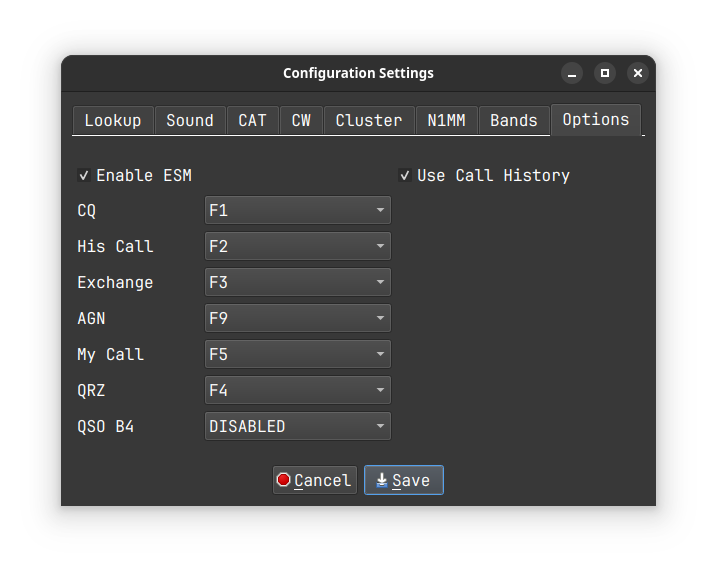
\includegraphics[width=0.9\linewidth]{pic/configuration_options.png}
\vspace{0.5cm}

Check the mark to Enable ESM and tell it which function keys do what. The keys will need to have the same function in both Run and S\&P modes. The function keys will highlight green depending on the state of the input fields. The green keys will be sent if you press the Enter key. You should use the Space bar to move to another field.

The contact will be automatically logged once all the needed info is collected and the QRZ (for Run) or Exchange (for S\&P) is sent.

\subsection{Run States}

\subsubsection{CQ}

\vspace{0.5cm}
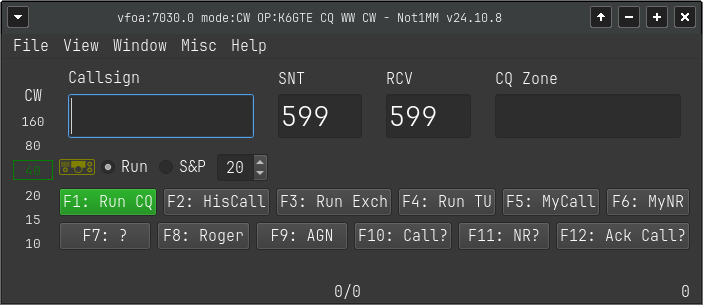
\includegraphics[width=0.75\linewidth]{pic/esm_cq.png}

\subsubsection{Call Entered Send His Call and the Exchange}

\vspace{0.5cm}
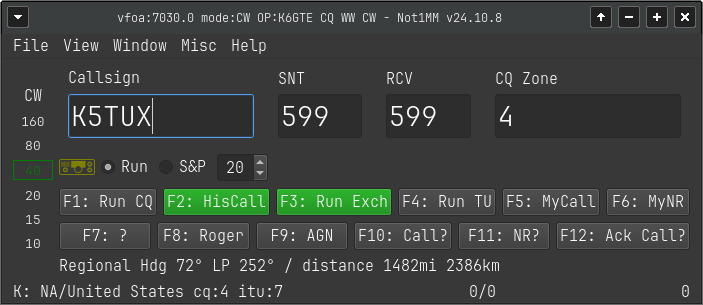
\includegraphics[width=0.75\linewidth]{pic/esm_withcall.png}

\subsubsection{Empty Exchange Field Send AGN Till You Get It}

\vspace{0.5cm}
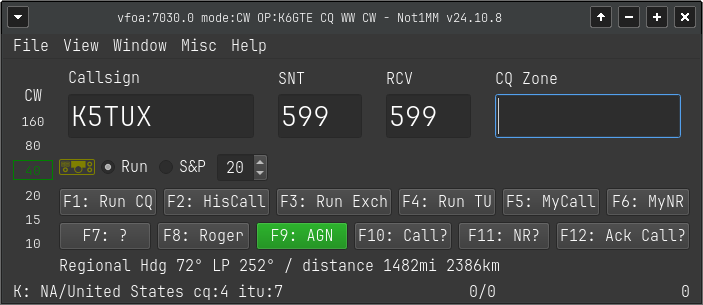
\includegraphics[width=0.75\linewidth]{pic/esm_empty_exchange.png}

\subsubsection{Exchange Field Filled, Send TU QRZ and Logs it}

\vspace{0.5cm}
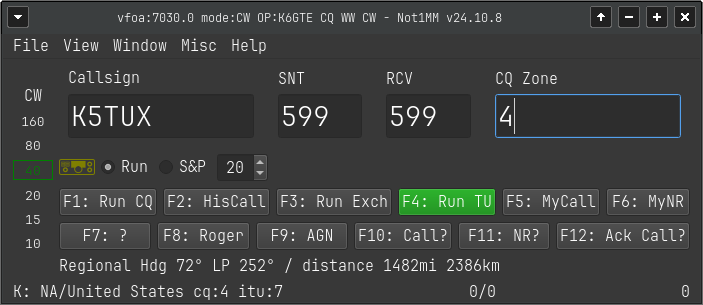
\includegraphics[width=0.75\linewidth]{pic/esm_qrz.png}

\subsection{S\&P States}

\subsubsection{With His Call Entered, Send Your Call}

\vspace{0.5cm}
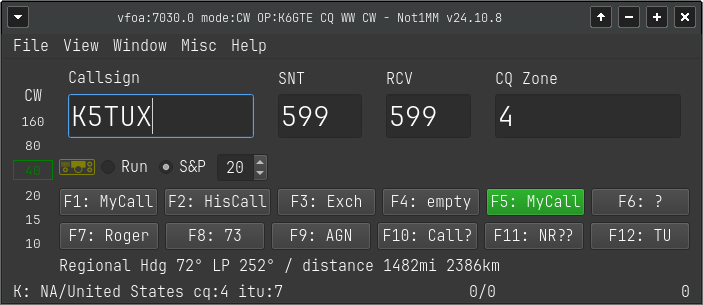
\includegraphics[width=0.75\linewidth]{pic/esm_sp_call.png}

\subsubsection{If No Exchange Entered Send AGN}

\vspace{0.5cm}
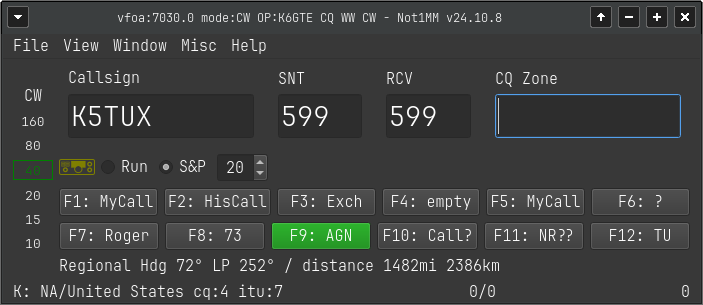
\includegraphics[width=0.75\linewidth]{pic/esm_sp_agn.png}

\subsubsection{With Exchange Entered, Send Your Exchange and Log it}

\vspace{0.5cm}
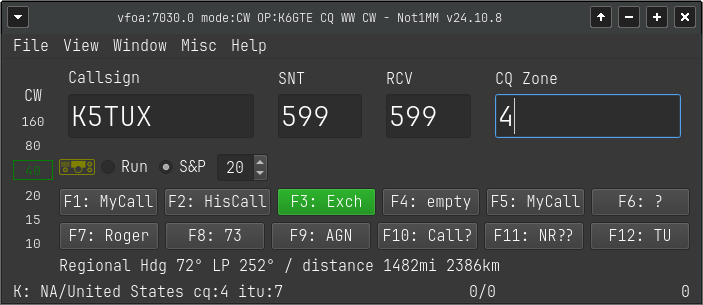
\includegraphics[width=0.75\linewidth]{pic/esm_sp_logit.png}
\newpage
\section{Call History Files}

To use Call History files, go to \textbf{FILE >> Configuration Settings}.

\vspace{0.5cm}
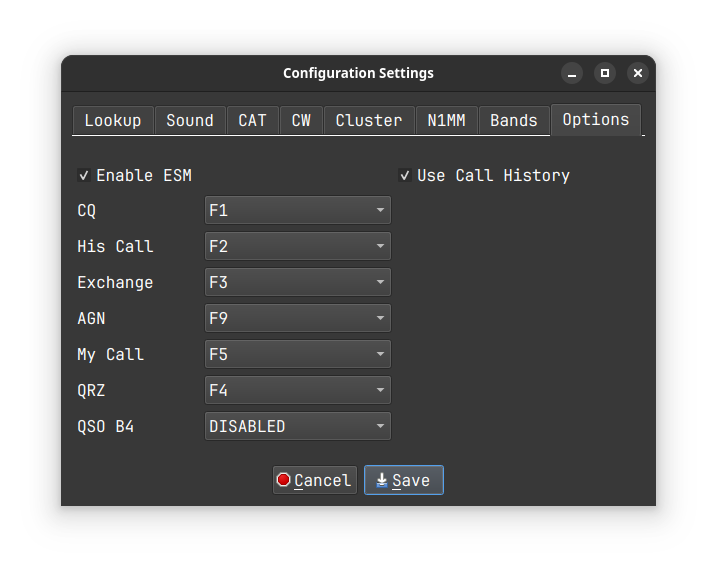
\includegraphics[width=0.9\linewidth]{pic/configuration_options.png}
\vspace{0.5cm}

Place a check in the `Use Call History` box. Call history files are very specific to the contest you are working. Example files can be obtained from https://n1mmwp.hamdocs.com/mmfiles/categories/callhistory/? website. They have a searchbox so you can find the contest you are looking for. If you are feeling masocistic, you can craft your own. The general makeup of the file is a header defining the fields to be used, followed by by lines of comma separated data.
\newpage
\section{Creating your own Call History files}
You can use \textbf{adif2callhistory} at 
\emph{https://github.com/mbridak/adif2callhistory} to generate your own call history file from your ADIF files.
An example file excerpt looks like:

\begin{verbatim}
!!Order!!,Call,Name,State,UserText,
#
# 0-This is helping file, LOG what is sent.
# 1-Last Edit,2024-08-18
# 2-Send any corrections direct to ve2fk@arrl.net
# 3-Updated from the log of Marsh/KA5M
# 4-Thanks Bjorn SM7IUN for his help.
# 5-Thanks
# NAQPCW
# NAQPRTTY
# NAQPSSB
# SPRINTCW
# SPRINTLADD
# SPRINTNS
# SPRINTRTTY
# SPRINTSSB
AA0AC,DAVE,MN,Example UserText
AA0AI,STEVE,IA,
AA0AO,TOM,MN,
AA0AW,DOUG,MN,
AA0BA,,TN,
AA0BR,,CO,
AA0BW,,MO,
\end{verbatim}
\newpage
The first line is the field definition header. The lines starting with a `\#` are comments. Some of the comments are other contests that this file also works with.
This is followed by the actual data. If the matched call has `UserText` information, that user text is populated to the bottom left of the logging window.

So if one were to go to \textbf{FILE >> LOAD CALL HISTORY FILE} and choose a downloaded call history file for NAQP and typed in the call AA0AC while operating in the NAQP, after pressing space, one would see:

\vspace{0.5cm}
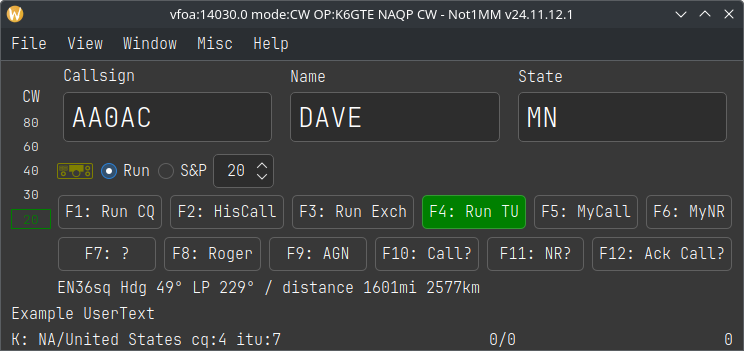
\includegraphics[width=0.9\linewidth]{pic/call_history_example.png}
\vspace{0.5cm}

Where the Name and State would auto-populate and the UserText info apprears in the bottom left.
\newpage
\section{Contest Specific Notes}

I found it might be beneficial to have a section devoted to wierd quirky things about operating a specific contests.

\subsection{ARRL Sweekstakes}

\subsubsection{The Exchange Parser}

This was a pain in the tukus. There are so many elements to the exchange, and one input field aside from the callsign field. So I had to write sort of a 'parser'. The parser moves over your input string following some basic rules and is re-evaluated with each keypress and the parsed result will be displayed in the label over the field. The exchange looks like `124 A K6GTE 17 ORG`, a Serial number, Precidence, Callsign, Year Licenced and Section. even though the callsign is given as part of the exchange, the callsign does not have to be entered and is pulled from the callsign field. If the exchange was entered as `124 A 17 ORG` you would see:

\vspace{0.5cm}
\includegraphics[width=0.5\linewidth]{pic/ss_parser_1.png}
\vspace{0.5cm}

You can enter the serial number and precidence, or the year and section as pairs. For instance `124A 17ORG`. This would ensure the values get parsed correctly.

You do not have to go back to correct typing. You can just tack the correct items to the end of the field and the older values will get overwritten. So if you entered `124A 17ORG Q`, the precidence will change from A to Q. If you need to change the serial number you must append the precidence to it, `125A`.

If the callsign was entered wrong in the callsign field, you can put the correct callsign some where in the exchange. As long as it shows up in the parsed label above correctly your good.

The best thing you can do is play around with it to see how it behaves.

\subsubsection{The Exchange}

In the `Sent Exchange` field of the New Contest dialog put in the Precidence, Call, Check and Section. Example: `A K6GTE 17 ORG`.

For the Run Exchange macro I'd put `{HISCALL} {SENTNR} {EXCH}`.

\subsection{RAEM}

In the New/Edit Contest dialog, in the exchange field put just your Lat and Lon. for me 33N117W. And in the exchange macro put `\# {EXCH}`.

\subsection{RandomGram}

This plugin was submitted by @alduhoo. It reads a rg.txt file if it exists in the user's home directory to populate the next group in the sent exchange field.

\subsection{UKEI DX}

For the Run exchange macro I'd put '{SNT} \# {EXCH}'

\subsection{CWO Open Contest}

Note: when completing the "Recd Number and Name" field, place a space between the received serial number and the name of the other operator. eg. "123 Fred". (Advance on spacebar is disabled for this field.)


\end{document}
